\section{Benutzerumfrage über die Feuerwehr-Community}

Ein wichtiger Aspekt der Silvanet-Anwendung ist die Benachrichtigung und Anzeige von Informationen über das Entstehen eines Waldbrandes und dessen Verfolgung in Echtzeit.
Es ist jedoch zu beachten, dass die Anwendung nicht für den Gebrauch durch Feuerwehrleute bestimmt ist.
Eine von Dryad im Vorfeld durchgeführte interne Untersuchung zeigte, dass die große Mehrheit der Feuerwehrleute seit vielen Jahren mit bestimmten Computer- oder anderen Lösungen arbeitet.
Der Versuch, mit dieser Gewohnheit durch eine noch so gut genutzte Anwendung zu konkurrieren, wäre also ein Misserfolg.

Die Anwendung beschränkt sich also darauf, die Informationen an den für den Standort verantwortlichen Kunden weiterzuleiten, der dann selbst die örtlichen Behörden und die Feuerwehr kontaktieren muss, die dann wie bisher die Arbeit übernehmen wird.
Die Feuerwehrleute, die auf den Platz gehen, sind nämlich nicht die Feuerwehrleute, die bei einem Notfall mit der Nummer 911 z. B. gerufen werden.
Diejenigen, die angerufen werden und die Informationen über den Notfall erhalten, heißen \textit{Dispatchers}.
Sie entscheiden anhand der erhaltenen Informationen, wie viele Einheiten wohin geschickt werden und leiten die Informationen an die Feuerwehrleute weiter, die vor Ort sind.
Eine Situation, in der ein Waldbrand entdeckt wird, kann also mit dem folgenden Use-Case-Diagramm schematisiert werden:

\begin{figure}[H]
  \centering
  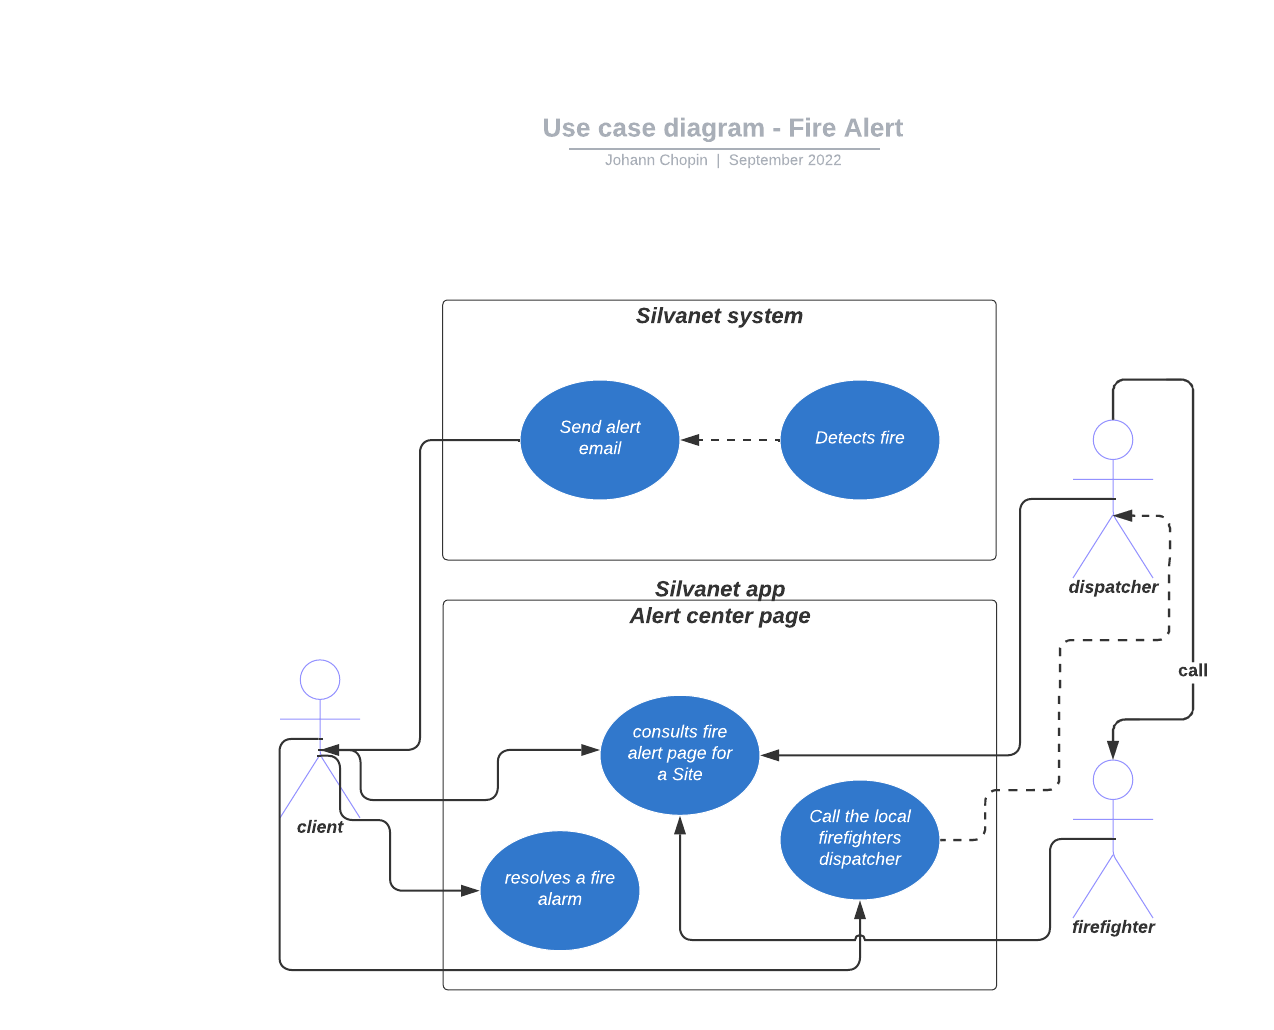
\includegraphics[width=\textwidth]{use_case_diagram_dispatcher}
  \caption{Use-case-diagram, das Kunden, Dispatchers, Feuerwehrleute, das Silvanet-System und die Silvanet-Anwendung bei der Erkennung eines Waldbrandes verbindet.}
  \label{fig:use_case_diagram_dispatcher}
\end{figure}
